%===============================================================================
% LOGFILE Developer Guide
%===============================================================================
% $Id: developer-guide.tex 231 2005-01-30 14:55:12Z thom $
%===============================================================================


%===============================================================================
% Configuration
%===============================================================================


%-------------------------------------------------------------------------------
% \documentclass and \usepackage directives
%-------------------------------------------------------------------------------
\documentclass[a4paper,fleqn,titlepage]{article}
%\usepackage{ngerman}
\usepackage[latin1]{inputenc}
\usepackage[T1]{fontenc}
\usepackage[small,hang,bf]{caption2}
\usepackage{fancyhdr}
\usepackage[nice]{nicefrac}
\usepackage{color,listings}
\usepackage{alltt}


% Compilation with latex or pdflatex?
\newif\ifpdf 
\ifx\pdfoutput\undefined 
  \pdffalse
\else
  \pdfoutput=1 
  \pdftrue 
\fi 

% Compilation with pdflatex
\ifpdf
 
  \usepackage[pdftex]{graphicx}

  \usepackage[
    pdftex,
    a4paper,
    bookmarks,
    pdfstartview=FitH,    % starts with page width
    bookmarksopen,        % opens index
    bookmarksnumbered,    % index with numbering
    colorlinks,           % links with color, otherwise with border
    linkcolor=blue,       % Standard red
    citecolor=blue,       % Standard green
    urlcolor=magenta,     % Standard cyan
    filecolor=blue
  ]{hyperref} 

  \pdfinfo{
    /Title      (EiffelRSS LOGFILE Developer Guide)
    /Author     (Thomas Weibel, Martin Luder, Michael K�ser)
    /Subject    (Eiffel programming)
    /Keywords   (Programming, EiffelRSS)
  }

  % Use default Acrobat reader fonts
  \usepackage{mathpazo}

  % Use CM fonts (increases document size)
  % \usepackage{ae}

% Compilation with latex
\else 

  \usepackage{graphicx} 

\fi


%-------------------------------------------------------------------------------
% Configure \maketitle
%-------------------------------------------------------------------------------
\title{EiffelRSS \\ LOGFILE \\ Developer Guide}
\author{
  Michael K\"aser <kaeserm@student.ethz.ch>
  \and 
  Martin Luder <luderm@student.ethz.ch>
  \and 
  Thomas Weibel <weibelt@student.ethz.ch>
}
\date{\today}


%-------------------------------------------------------------------------------
% Configure fancyhdr
%-------------------------------------------------------------------------------
\pagestyle{fancy}

\renewcommand{\headrulewidth}{0.1 pt}
\renewcommand{\footrulewidth}{0.1 pt}

\fancypagestyle{plain}{
  \lhead{\nouppercase{\leftmark}}
  \chead{}
  \rhead{\thepage}
  \lfoot{EiffelRSS}
  \cfoot{}
  \rfoot{LOGFILE Developer Guide}
}

\lhead{\nouppercase{\leftmark}}
\chead{}
\rhead{\thepage}

\lfoot{EiffelRSS}
\cfoot{}
\rfoot{LOGFILE Developer Guide}


%-------------------------------------------------------------------------------
% Configure listings
%-------------------------------------------------------------------------------
\lstset{showstringspaces=false,
  breaklines=true,
  breakindent=0pt,
  prebreak=\mbox{\tiny$\searrow$},
  postbreak=\mbox{{\color{blue}\tiny$\rightarrow$}},
  frame=trBL,
  framerule=0.75pt,
  framesep=4pt,
  rulesep=0.75pt  
}


%-------------------------------------------------------------------------------
% Common configuration
%-------------------------------------------------------------------------------
\setlength{\parindent}{0em}
\setlength{\parskip}{1.5ex plus0.5ex minus0.5ex}
\sloppy
\setlength{\mathindent}{0em}


%-------------------------------------------------------------------------------
% Commandos
%-------------------------------------------------------------------------------
\newcommand{\hr}{\rule{\textwidth}{1pt}}


%===============================================================================
% Document
%===============================================================================
\begin{document}

\begin{titlepage}
  \newlength{\centeroffset}
  \setlength{\centeroffset}{-0.5\oddsidemargin}
  \addtolength{\centeroffset}{0.5\evensidemargin}

  \thispagestyle{empty}

  \noindent
\includegraphics[width=\textwidth]{../../figures/big_ETH}\\[-3mm]
  \hr

  \vspace*{\stretch{1}}

  \makebox[0pt][l]{
    \begin{minipage}{\textwidth}
      \flushright{
        \Huge\bfseries EiffelRSS
      }

      \noindent\rule{\textwidth}{3pt}\\[2.5ex]

      \hfill\emph{
        \Large LOGFILE Developer Guide
      }
    \end{minipage}
  }

  \vspace{\stretch{1}}

  \makebox[0pt][l]{
    \begin{minipage}{\textwidth}
      \flushright{
        \bfseries 
        Michael K\"aser <kaeserm@student.ethz.ch>\\[0.3ex]
        Martin Luder <luderm@student.ethz.ch>\\[0.3ex]
        Thomas Weibel <weibelt@student.ethz.ch>\\[0.3ex]
      }
    \end{minipage}
  }

  \vspace{\stretch{1}}

  \noindent\hr\\[1mm]
  
\includegraphics[width=\textwidth]{../../figures/big_inf}
\end{titlepage}

% Use roman page numbering
\pagenumbering{roman}

\begin{abstract}
  \texttt{LOGFILE} represents a file which can be used for logging
  messages during the program execution.
\end{abstract}

\clearpage
\tableofcontents

\clearpage
\listoffigures

\newpage

\section{Overview}
\label{sec:overview}

% Set page counter to zero
\setcounter{page}{0} 

% Use arabic page numbering
\pagenumbering{arabic}

\texttt{LOGFILE} represents a file which can be used for logging
messages during the program execution.

Each message has its own priority (a positive integer value) and each
logfile a certain user defined threshold. If the priority of the
message is greater or equal than the threshold, it gets written to the
log file together with a timestamp.

See figure \ref{fig:cluster} for an overview of the cluster.

\begin{figure}[htbp]
  \centering
  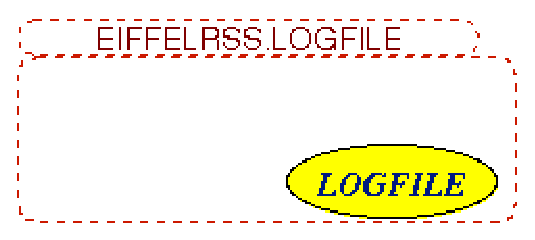
\includegraphics[scale=.6]{./figures/EIFFELRSS_LOGFILE}
  \caption{BON diagram of cluster \texttt{LOGFILE}}
  \label{fig:cluster}
\end{figure}

Figure \ref{fig:classes} shows the class \texttt{LOGFILE}.

\begin{figure}[htbp]
  \centering
  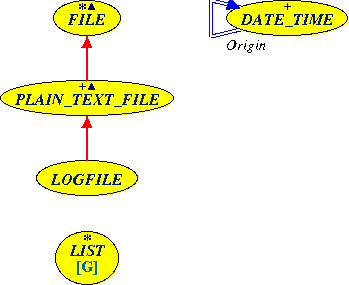
\includegraphics[scale=.6]{./figures/LOGFILE}
  \caption{BON diagram of class \texttt{LOGFILE}}
  \label{fig:classes}
\end{figure}

\newpage

\section{Usage}
\label{sec:usage}

\begin{lstlisting}[language=Eiffel]
class USAGE_EXAMPLE

create make

feature -- Initialization

  make is
      -- Creation procedure.
    do                  
      -- Create logfile
      create log_file.make_filename("logfile")

      -- Set the threshold
      log_file.set_threshold(log_file.Error)
                        
      -- Output a message with one line and priority critical
      log_file.log_message("One line test message", log_file.Critical)

      -- Output a message which won't be logged
      log_file.log_message("Not important enough", log_file.Info)

      -- Output a multi-line message
      log_file.log_message("Line One%NLine Two%NLine Three", log_file.Error)
    end
                
feature -- Arguments

  log_file: LOGFILE
      -- Logfile
        
end -- class USAGE_EXAMPLE
\end{lstlisting}

The output of the above example is

\begin{lstlisting}
[16:02:37 05 JAN 2005]: One line test message
[16:02:37 05 JAN 2005]: Line One
                        Line Two
                        Line Three
\end{lstlisting}


\section{Features}
\label{sec:features}


\subsection{Initialization}
\label{sec:initialization}


\subsubsection{make\_filename}

\begin{lstlisting}[language=Eiffel]
make_filename (a_filename: STRING) is
  -- Create logfile object with a_filename as file name
\end{lstlisting}

Note that the default threshold which will be set if you create the
object with this procedure is zero.


\subsubsection{make\_filename\_threshold}

\begin{lstlisting}[language=Eiffel]
make_filename_threshold (a_filename: STRING; a_threshold: INTEGER) is
  -- Create logfile object with a_filename as file name and a_threshold as output threshold
\end{lstlisting}


\subsection{Access}
\label{sec:access}


\subsubsection{messages\_logged}

\begin{lstlisting}[language=Eiffel]
messages_logged: INTEGER
  -- The number of messages which got logged
\end{lstlisting}


\subsubsection{output\_threshold}

\begin{lstlisting}[language=Eiffel]
output_threshold: INTEGER
  -- The current threshold used
\end{lstlisting}


\subsection{Constants}
\label{sec:Constants}

\begin{lstlisting}[language=Eiffel]
Developer, Info, Notice, Warning, Error, Critical, Alert, Emerge: INTEGER is unique
  -- Some predefined constants which can be used as a priority
\end{lstlisting}


\subsection{Basic Operations}
\label{sec:Basic Operations}

\subsubsection{set\_threshold}

\begin{lstlisting}[language=Eiffel]
set_threshold (a_threshold: INTEGER) is
  -- Set the output threshold to a_threshold
\end{lstlisting}

Sets a new threshold, which must be a positive integer value. Each
message which the object receives after the execution of this command
is only written to the logfile if its priority is greater or equal the
threshold.


\subsubsection{log\_message}

\begin{lstlisting}[language=Eiffel]
log_message (a_message: STRING; a_priority: INTEGER) is
  -- Log the message to the logfile if a_priority is equal or greater than the threshold
\end{lstlisting}

This is the actual command to send a message to the object. If the
priority is high enough, a timestamp with format

\begin{lstlisting}
  [[0]hh:[0]mi:[0]ss [0]dd mmm yyyy]:
\end{lstlisting}

gets added. If the message containts line breaks, all lines will get
correctly indented.

\textit{\textbf{Attention:}} Note that there is no guarantee that the
operating system will physically write the data to the disk. At least
it will end up in the buffer cache, making the data visible to other
processes.

\end{document}
